\graphicspath{{fig/scoters/}}

\chapter{Case Study II: Foraging Scoters}
\label{cha:scoters}

In the previous chapter we discussed how data could easily go missing during
flocking events. In \emph{this} chapter we shall consider a real dataset with
missing observations. As foreshadowed in the previous chapter, the missing
observations of this dataset are a product of employing fixed-location
recording equipment.

This dataset details the movements of a large number of surf scoters, a
migratory sea bird, which gather in groups to forage. The captured flocking
events take place on the surface of a lake, and so movement is effectively
restricted to a two-dimensional plane. This dataset was provided courtesy of
work performed by \textcite{lukeman09,lukeman10}, at the time representing a
tenfold increase in the number of individuals which could be reliably tracked
between frames.

Unfortunately, owing to the fixed location cameras used to record these
flocking events, there were often scoters out of view during recorded frames.
This can be seen by considering the images of extracted frames in
\cref{fig:lukeman_extraction}. As in \cref{cha:missing}, the missing
data points can be partitioned into observations missing at the beginning of
the recording event, and observations missing at the end of the recording
event.

In this chapter we shall fit a simple variation of the Vicsek model to
flocking events of this dataset. The missing data points will be integrated out
of the problem, using the methodology developed in \cref{cha:missing}.

\section{Scoter data}

\textcite{lukeman10} captured their flocking events from an aerial vantage
point: an elevated promenade at the side of a large lake. From this position
the authors were able to direct a camera toward an inlet where overwintering
scoters had been observed foraging. Knowing the height of this camera above the
water, and its angle against the horizontal, the authors were able to transform
the captured camera data back to `real-world' co-ordinates.

However, to reliably transform back from the camera co-ordinates to real-world
co-ordinates, the height of the camera above the lake and its angle of approach
had to be fixed. With the camera fixed in position, the authors then waited for
flocking events to occur. Recording began when individuals entered the camera's
field of vision, and ceased when all the individuals left the frame, or became
stationary.

Each recording event captured the movements of $\approx170$ scoters,
with each event lasting for $\approx30$ frames. However, for these sequences
between $16\%$ and $64\%$ of the data points were missing.

\textcite{lukeman10} discounted the influence of individuals out-of-frame, and
instead focussed on reproducing radial and nearest neighbour distributions of
\emph{internal} group members. This approach, although representing a
\emph{significant} step forward in the literature, came with its drawbacks.
Most significantly, focussing the fitting on reproducing nearest-neighbour and
radial neighbour distributions removed the \emph{dynamic} component to the data
which the authors worked so hard to achieve.

Here we take a more holistic approach to model fitting; making sure to account
for all individuals---both observed and missing---and focussing the fitting on
reproducing the \emph{movements} of the individuals, rather than some
epiphenomena of the movements. With the additional demand of inferring
posterior distributions of parameters, rather than simple point estimates, this
approach will represent a more computationally demanding problem than that
faced by the original authors. As such, here we will be fitting a model simpler
than that considered by \textcite{lukeman10}.

In \cref{cha:missing} we discussed how the computational load of our inference
scheme increases as the number of missing observations increases. With this in
mind we shall be focussing on events with the \emph{fewest} number of missing
observations. For the events captured by \textcite{lukeman10} this is
represented by a sequence of $199$ agents moving over $23$ frames. Of the
$199\times23=4577$ data points represented by this event, $680$ ($\approx16\%)$
of these observations are out of frame. This event is visualised in
\cref{fig:scoter_traj}.

\begin{figure}[tb]
  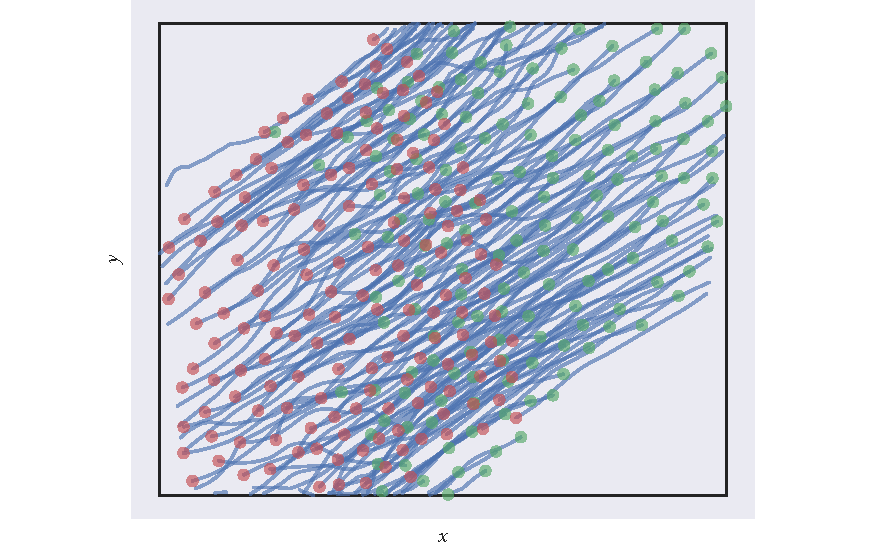
\includegraphics{data_00_traj.pdf}
  \caption{A visualisation of the trajectories of foraging scoters. The scoters
  move along the blue trajectories, starting from the positions denoted by the
  green markers and finishing at the positions shown by the red markers. The
  black frame containing the trajectories represents the fixed field of vision
  of the recording equipment.}
  \label{fig:scoter_traj}
\end{figure}

The simulated flocks considered in \cref{cha:missing} had between $10$ and $20$
missing observations per sequence. With $680$ data points missing from the
scoter sequence with the \emph{least} amount of missingness, this problem
represents a considerable increase in complexity. With this amount of
missingness, long and expensive simulations will be necessary to realise a
satisfactory number of samples from the posterior.

\begin{figure}[tb]
  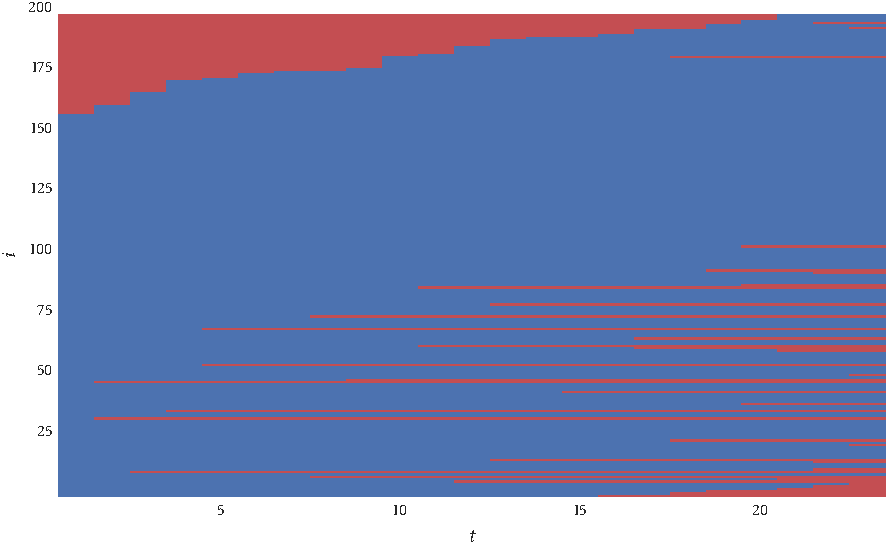
\includegraphics{data_00_missing.pdf}
  \caption{A representation of the missing and observed data points of the
  foraging event shown in \cref{fig:scoter_traj}. The $x$-axis represents the
  frame of the sequence, and the $y$-axis corresponds to tracked individuals. A
  blue tile at location $(i,t)$ tells us that scoter $i$ was observed in frame
  $t$. A red tile at $(i,t)$ indicates that scoter $i$ was missing at time $t$.}
  \label{fig:scoter_missing}
\end{figure}

In \cref{cha:missing} we used summary plots---such as those in
\cref{fig:beg_summary,fig:end_summary}---to help visualise high-dimensional
posterior distributions. However, with $680$ dimensions (plus a few extra for
the model parameters), this posterior has too many dimensions for even these
summary plots. In such a situation it can be informative to graphically assess
the convergence of the log-likelihood. If we can observe that the
log-likelihood has converged, we have good evidence that all the remaining
parameters have also converged.

\begin{figure}[tb]
  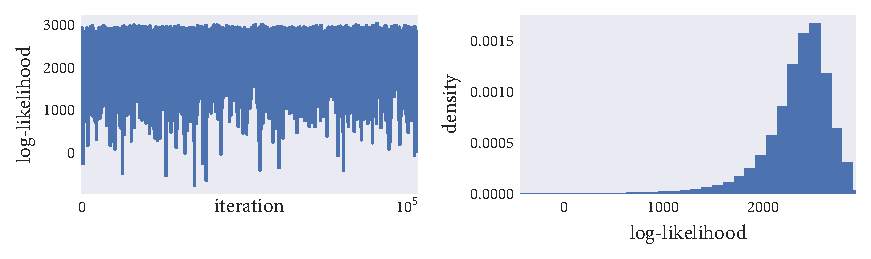
\includegraphics{log_likelihood.pdf}
  \caption{Trace and histogram plots of the log-likelihood, as computed at
    every iteration of the inference scheme. As it can be difficult to assess
    the convergence of all the parameters for high-dimensional problems, as we have
    here, it can instead be informative to assess the convergence of the
    log-likelihood. If we see that the value of the log-likelihood has
    converged, then we have evidence that the corresponding parameters also
    converged.}
\end{figure}

\begin{figure}[tb]
  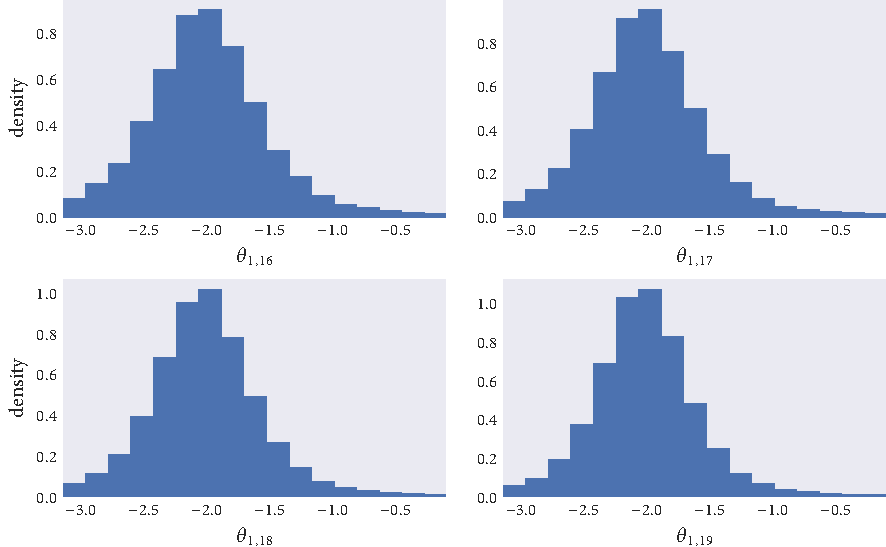
\includegraphics{dir_hist.pdf}
  \caption{Histogram plots of posterior draws of $4$ missing directions (out of
  a total of $680$) missing data points.}
  \label{fig:dir_hist}
\end{figure}

\begin{figure}[tb]
  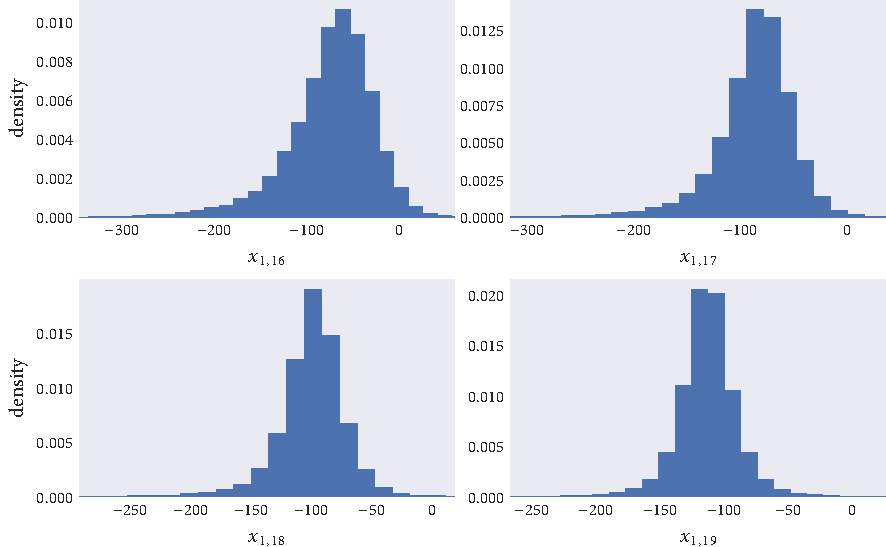
\includegraphics{x_hist.pdf}
  \caption{}
  \label{fig:x_hist}
\end{figure}










